 \begin{figure}[H]
  \centering
  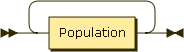
\includegraphics[resolution=120,max size={\textwidth}{\textheight}]
  {Figures/Ebnf/Populations}
  \caption*{Populations \small::=  Population+}
  \label{fig:ebnf-Populations}
 \end{figure}

 \begin{figure}[H]
  \centering
  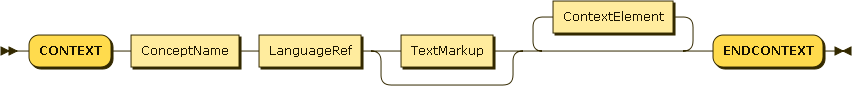
\includegraphics[resolution=120,max size={\textwidth}{\textheight}]
  {Figures/Ebnf/Context}
  \caption*{Context \small::=  'CONTEXT' ConceptName LanguageRef TextMarkup? ContextElement* 'ENDCONTEXT'}
  \label{fig:ebnf-Context}
 \end{figure}

 \begin{figure}[H]
  \centering
  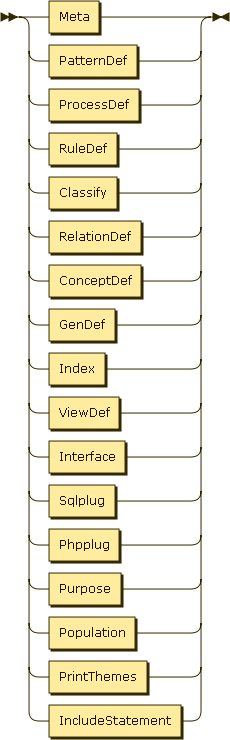
\includegraphics[resolution=120,max size={\textwidth}{\textheight}]
  {Figures/Ebnf/ContextElement}
  \caption*{ContextElement \small::=  Meta | PatternDef | ProcessDef | RuleDef | Classify | RelationDef | ConceptDef | GenDef | Index | ViewDef | Interface | Sqlplug | Phpplug | Purpose | Population | PrintThemes | IncludeStatement}
  \label{fig:ebnf-ContextElement}
 \end{figure}

 \begin{figure}[H]
  \centering
  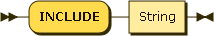
\includegraphics[resolution=120,max size={\textwidth}{\textheight}]
  {Figures/Ebnf/IncludeStatement}
  \caption*{IncludeStatement \small::=  'INCLUDE' String}
  \label{fig:ebnf-IncludeStatement}
 \end{figure}

 \begin{figure}[H]
  \centering
  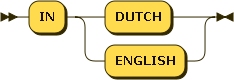
\includegraphics[resolution=120,max size={\textwidth}{\textheight}]
  {Figures/Ebnf/LanguageRef}
  \caption*{LanguageRef \small::=  'IN' ('DUTCH' | 'ENGLISH')}
  \label{fig:ebnf-LanguageRef}
 \end{figure}

 \begin{figure}[H]
  \centering
  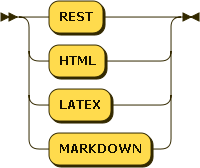
\includegraphics[resolution=120,max size={\textwidth}{\textheight}]
  {Figures/Ebnf/TextMarkup}
  \caption*{TextMarkup \small::=  'REST' | 'HTML' | 'LATEX' | 'MARKDOWN'}
  \label{fig:ebnf-TextMarkup}
 \end{figure}

 \begin{figure}[H]
  \centering
  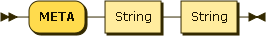
\includegraphics[resolution=120,max size={\textwidth}{\textheight}]
  {Figures/Ebnf/Meta}
  \caption*{Meta \small::=  'META' String String}
  \label{fig:ebnf-Meta}
 \end{figure}

 \begin{figure}[H]
  \centering
  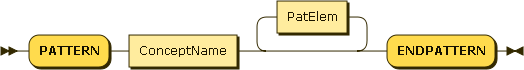
\includegraphics[resolution=120,max size={\textwidth}{\textheight}]
  {Figures/Ebnf/PatternDef}
  \caption*{PatternDef \small::=  'PATTERN' ConceptName PatElem* 'ENDPATTERN'}
  \label{fig:ebnf-PatternDef}
 \end{figure}

 \begin{figure}[H]
  \centering
  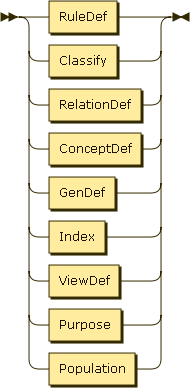
\includegraphics[resolution=120,max size={\textwidth}{\textheight}]
  {Figures/Ebnf/PatElem}
  \caption*{PatElem \small::=  RuleDef | Classify | RelationDef | ConceptDef | GenDef | Index | ViewDef | Purpose | Population}
  \label{fig:ebnf-PatElem}
 \end{figure}

 \begin{figure}[H]
  \centering
  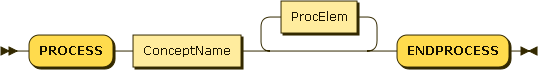
\includegraphics[resolution=120,max size={\textwidth}{\textheight}]
  {Figures/Ebnf/ProcessDef}
  \caption*{ProcessDef \small::=  'PROCESS' ConceptName ProcElem* 'ENDPROCESS'}
  \label{fig:ebnf-ProcessDef}
 \end{figure}

 \begin{figure}[H]
  \centering
  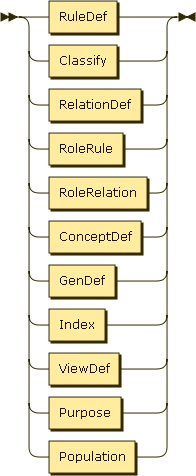
\includegraphics[resolution=120,max size={\textwidth}{\textheight}]
  {Figures/Ebnf/ProcElem}
  \caption*{ProcElem \small::=  RuleDef | Classify | RelationDef | RoleRule | RoleRelation | ConceptDef | GenDef | Index | ViewDef | Purpose | Population}
  \label{fig:ebnf-ProcElem}
 \end{figure}

 \begin{figure}[H]
  \centering
  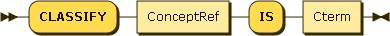
\includegraphics[resolution=120,max size={\textwidth}{\textheight}]
  {Figures/Ebnf/Classify}
  \caption*{Classify \small::=  'CLASSIFY' ConceptRef 'IS' Cterm}
  \label{fig:ebnf-Classify}
 \end{figure}

 \begin{figure}[H]
  \centering
  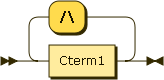
\includegraphics[resolution=120,max size={\textwidth}{\textheight}]
  {Figures/Ebnf/Cterm}
  \caption*{Cterm \small::=  Cterm1 ('/\' Cterm1)*}
  \label{fig:ebnf-Cterm}
 \end{figure}

 \begin{figure}[H]
  \centering
  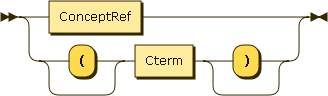
\includegraphics[resolution=120,max size={\textwidth}{\textheight}]
  {Figures/Ebnf/Cterm1}
  \caption*{Cterm1 \small::=  ConceptRef | ('('? Cterm ')'?)}
  \label{fig:ebnf-Cterm1}
 \end{figure}

 \begin{figure}[H]
  \centering
  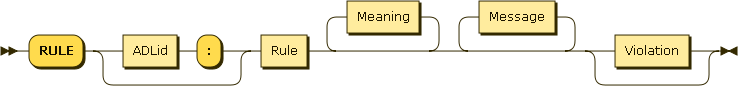
\includegraphics[resolution=120,max size={\textwidth}{\textheight}]
  {Figures/Ebnf/RuleDef}
  \caption*{RuleDef \small::=  'RULE' (ADLid ':')? Rule Meaning* Message* Violation?}
  \label{fig:ebnf-RuleDef}
 \end{figure}

 \begin{figure}[H]
  \centering
  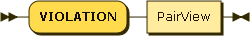
\includegraphics[resolution=120,max size={\textwidth}{\textheight}]
  {Figures/Ebnf/Violation}
  \caption*{Violation \small::=  'VIOLATION' PairView}
  \label{fig:ebnf-Violation}
 \end{figure}

 \begin{figure}[H]
  \centering
  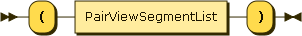
\includegraphics[resolution=120,max size={\textwidth}{\textheight}]
  {Figures/Ebnf/PairView}
  \caption*{PairView \small::=  '(' PairViewSegmentList ')'}
  \label{fig:ebnf-PairView}
 \end{figure}

 \begin{figure}[H]
  \centering
  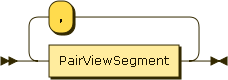
\includegraphics[resolution=120,max size={\textwidth}{\textheight}]
  {Figures/Ebnf/PairViewSegmentList}
  \caption*{PairViewSegmentList \small::=  PairViewSegment (',' PairViewSegment)*}
  \label{fig:ebnf-PairViewSegmentList}
 \end{figure}

 \begin{figure}[H]
  \centering
  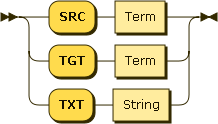
\includegraphics[resolution=120,max size={\textwidth}{\textheight}]
  {Figures/Ebnf/PairViewSegment}
  \caption*{PairViewSegment \small::=  'SRC' Term | 'TGT' Term | 'TXT' String}
  \label{fig:ebnf-PairViewSegment}
 \end{figure}

 \begin{figure}[H]
  \centering
  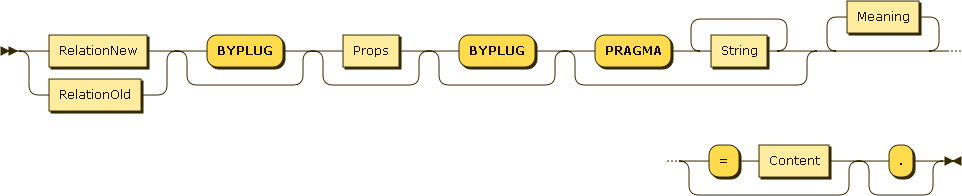
\includegraphics[resolution=120,max size={\textwidth}{\textheight}]
  {Figures/Ebnf/RelationDef}
  \caption*{RelationDef \small::=  (RelationNew | RelationOld) 'BYPLUG'? Props? 'BYPLUG'? ('PRAGMA' String+)? Meaning* ('=' Content)? '.'?}
  \label{fig:ebnf-RelationDef}
 \end{figure}

 \begin{figure}[H]
  \centering
  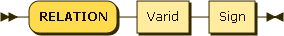
\includegraphics[resolution=120,max size={\textwidth}{\textheight}]
  {Figures/Ebnf/RelationNew}
  \caption*{RelationNew \small::=  'RELATION' Varid Sign}
  \label{fig:ebnf-RelationNew}
 \end{figure}

 \begin{figure}[H]
  \centering
  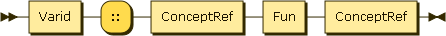
\includegraphics[resolution=120,max size={\textwidth}{\textheight}]
  {Figures/Ebnf/RelationOld}
  \caption*{RelationOld \small::=  Varid '::' ConceptRef Fun ConceptRef}
  \label{fig:ebnf-RelationOld}
 \end{figure}

 \begin{figure}[H]
  \centering
  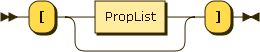
\includegraphics[resolution=120,max size={\textwidth}{\textheight}]
  {Figures/Ebnf/Props}
  \caption*{Props \small::=  '[' PropList? ']'}
  \label{fig:ebnf-Props}
 \end{figure}

 \begin{figure}[H]
  \centering
  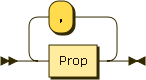
\includegraphics[resolution=120,max size={\textwidth}{\textheight}]
  {Figures/Ebnf/PropList}
  \caption*{PropList \small::=  Prop (',' Prop)*}
  \label{fig:ebnf-PropList}
 \end{figure}

 \begin{figure}[H]
  \centering
  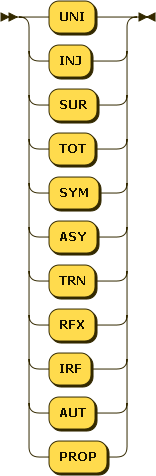
\includegraphics[resolution=120,max size={\textwidth}{\textheight}]
  {Figures/Ebnf/Prop}
  \caption*{Prop \small::=  'UNI' | 'INJ' | 'SUR' | 'TOT' | 'SYM' | 'ASY' | 'TRN' | 'RFX' | 'IRF' | 'AUT' | 'PROP'}
  \label{fig:ebnf-Prop}
 \end{figure}

 \begin{figure}[H]
  \centering
  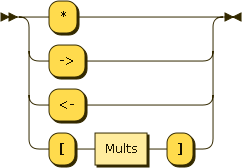
\includegraphics[resolution=120,max size={\textwidth}{\textheight}]
  {Figures/Ebnf/Fun}
  \caption*{Fun \small::=  '*' | '->' | '<-' | '[' Mults ']'}
  \label{fig:ebnf-Fun}
 \end{figure}

 \begin{figure}[H]
  \centering
  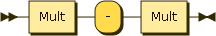
\includegraphics[resolution=120,max size={\textwidth}{\textheight}]
  {Figures/Ebnf/Mults}
  \caption*{Mults \small::=  Mult '-' Mult}
  \label{fig:ebnf-Mults}
 \end{figure}

 \begin{figure}[H]
  \centering
  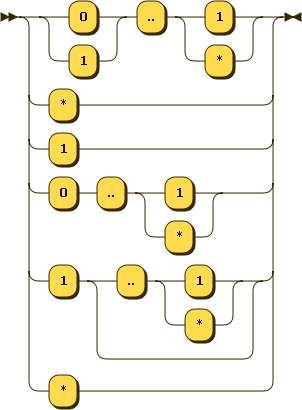
\includegraphics[resolution=120,max size={\textwidth}{\textheight}]
  {Figures/Ebnf/Mult}
  \caption*{Mult \small::=  ('0' | '1') '..' ('1' | '*') | '*' | '1'}
  \label{fig:ebnf-Mult}
 \end{figure}

 \begin{figure}[H]
  \centering
  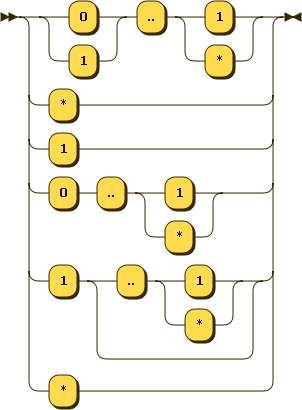
\includegraphics[resolution=120,max size={\textwidth}{\textheight}]
  {Figures/Ebnf/Mult}
  \caption*{Mult \small::=  '0' '..' ('1' | '*') | '1'('..' ('1' | '*'))? | '*'}
  \label{fig:ebnf-Mult}
 \end{figure}

 \begin{figure}[H]
  \centering
  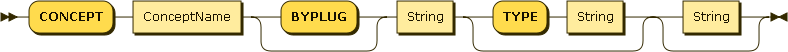
\includegraphics[resolution=120,max size={\textwidth}{\textheight}]
  {Figures/Ebnf/ConceptDef}
  \caption*{ConceptDef \small::=  'CONCEPT' ConceptName 'BYPLUG'? String ('TYPE' String)? String?}
  \label{fig:ebnf-ConceptDef}
 \end{figure}

 \begin{figure}[H]
  \centering
  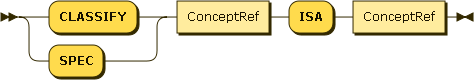
\includegraphics[resolution=120,max size={\textwidth}{\textheight}]
  {Figures/Ebnf/GenDef}
  \caption*{GenDef \small::=  ('CLASSIFY' | 'SPEC') ConceptRef 'ISA' ConceptRef}
  \label{fig:ebnf-GenDef}
 \end{figure}

 \begin{figure}[H]
  \centering
  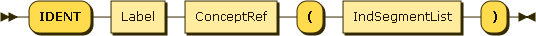
\includegraphics[resolution=120,max size={\textwidth}{\textheight}]
  {Figures/Ebnf/Index}
  \caption*{Index \small::=  'IDENT' Label ConceptRefPos '(' IndSegmentList ')'}
  \label{fig:ebnf-Index}
 \end{figure}

 \begin{figure}[H]
  \centering
  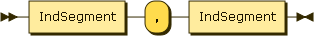
\includegraphics[resolution=120,max size={\textwidth}{\textheight}]
  {Figures/Ebnf/IndSegmentList}
  \caption*{IndSegmentList \small::=  IndSegment (',' IndSegment)}
  \label{fig:ebnf-IndSegmentList}
 \end{figure}

 \begin{figure}[H]
  \centering
  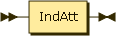
\includegraphics[resolution=120,max size={\textwidth}{\textheight}]
  {Figures/Ebnf/IndSegment}
  \caption*{IndSegment \small::=  IndAtt}
  \label{fig:ebnf-IndSegment}
 \end{figure}

 \begin{figure}[H]
  \centering
  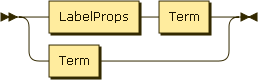
\includegraphics[resolution=120,max size={\textwidth}{\textheight}]
  {Figures/Ebnf/IndAtt}
  \caption*{IndAtt \small::=  LabelProps Term | Term}
  \label{fig:ebnf-IndAtt}
 \end{figure}

 \begin{figure}[H]
  \centering
  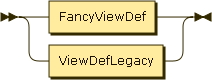
\includegraphics[resolution=120,max size={\textwidth}{\textheight}]
  {Figures/Ebnf/ViewDef}
  \caption*{ViewDef \small::=  FancyViewDef | ViewDefLegacy}
  \label{fig:ebnf-ViewDef}
 \end{figure}

 \begin{figure}[H]
  \centering
  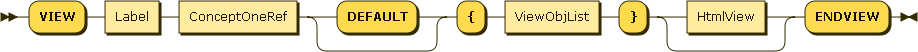
\includegraphics[resolution=120,max size={\textwidth}{\textheight}]
  {Figures/Ebnf/FancyViewDef}
  \caption*{FancyViewDef \small::=  'VIEW' pLabel ConceptOneRefPos 'DEFAULT'? '{' ViewObjList '}' HtmlView? 'ENDVIEW'}
  \label{fig:ebnf-FancyViewDef}
 \end{figure}

 \begin{figure}[H]
  \centering
  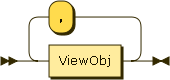
\includegraphics[resolution=120,max size={\textwidth}{\textheight}]
  {Figures/Ebnf/ViewObjList}
  \caption*{ViewObjList \small::=  ViewObj (',' ViewObj)*}
  \label{fig:ebnf-ViewObjList}
 \end{figure}

 \begin{figure}[H]
  \centering
  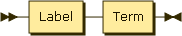
\includegraphics[resolution=120,max size={\textwidth}{\textheight}]
  {Figures/Ebnf/ViewObj}
  \caption*{ViewObj \small::=  Label Term}
  \label{fig:ebnf-ViewObj}
 \end{figure}

 \begin{figure}[H]
  \centering
  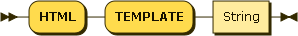
\includegraphics[resolution=120,max size={\textwidth}{\textheight}]
  {Figures/Ebnf/HtmlView}
  \caption*{HtmlView \small::=  'HTML' 'TEMPLATE' String}
  \label{fig:ebnf-HtmlView}
 \end{figure}

 \begin{figure}[H]
  \centering
  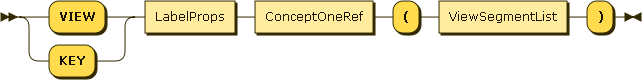
\includegraphics[resolution=120,max size={\textwidth}{\textheight}]
  {Figures/Ebnf/ViewDefLegacy}
  \caption*{ViewDefLegacy \small::=  ('VIEW' | 'KEY') LabelProps ConceptOneRefPos '(' ViewSegmentList ')'}
  \label{fig:ebnf-ViewDefLegacy}
 \end{figure}

 \begin{figure}[H]
  \centering
  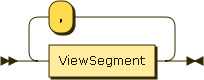
\includegraphics[resolution=120,max size={\textwidth}{\textheight}]
  {Figures/Ebnf/ViewSegmentList}
  \caption*{ViewSegmentList \small::=  ViewSegment (',' ViewSegment)*}
  \label{fig:ebnf-ViewSegmentList}
 \end{figure}

 \begin{figure}[H]
  \centering
  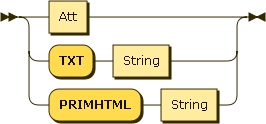
\includegraphics[resolution=120,max size={\textwidth}{\textheight}]
  {Figures/Ebnf/ViewSegment}
  \caption*{ViewSegment \small::=  ViewAtt | 'TXT' String | 'PRIMHTML' String}
  \label{fig:ebnf-ViewSegment}
 \end{figure}

 \begin{figure}[H]
  \centering
  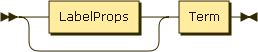
\includegraphics[resolution=120,max size={\textwidth}{\textheight}]
  {Figures/Ebnf/ViewAtt}
  \caption*{ViewAtt \small::=  LabelProps? Term}
  \label{fig:ebnf-ViewAtt}
 \end{figure}

 \begin{figure}[H]
  \centering
  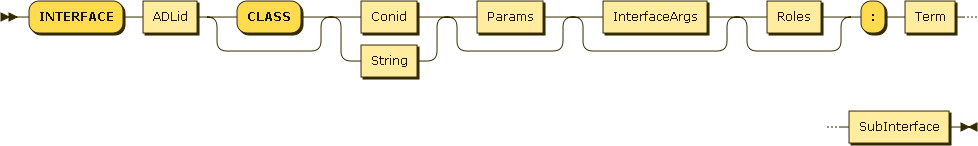
\includegraphics[resolution=120,max size={\textwidth}{\textheight}]
  {Figures/Ebnf/Interface}
  \caption*{Interface \small::=  'INTERFACE' ADLid 'CLASS'? (Conid | String) Params? InterfaceArgs? Roles? ':' Term SubInterface}
  \label{fig:ebnf-Interface}
 \end{figure}

 \begin{figure}[H]
  \centering
  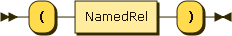
\includegraphics[resolution=120,max size={\textwidth}{\textheight}]
  {Figures/Ebnf/Params}
  \caption*{Params \small::=  '(' NamedRel ')'}
  \label{fig:ebnf-Params}
 \end{figure}

 \begin{figure}[H]
  \centering
  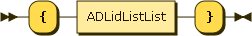
\includegraphics[resolution=120,max size={\textwidth}{\textheight}]
  {Figures/Ebnf/InterfaceArgs}
  \caption*{InterfaceArgs \small::=  '{' ADLidListList '}'}
  \label{fig:ebnf-InterfaceArgs}
 \end{figure}

 \begin{figure}[H]
  \centering
  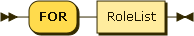
\includegraphics[resolution=120,max size={\textwidth}{\textheight}]
  {Figures/Ebnf/Roles}
  \caption*{Roles \small::=  'FOR' RoleList}
  \label{fig:ebnf-Roles}
 \end{figure}

 \begin{figure}[H]
  \centering
  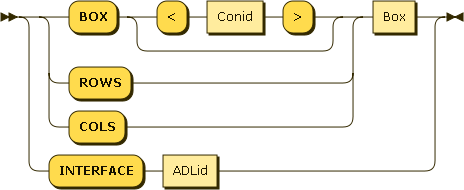
\includegraphics[resolution=120,max size={\textwidth}{\textheight}]
  {Figures/Ebnf/SubInterface}
  \caption*{SubInterface \small::=  ('BOX' ('<' Conid '>')? | 'ROWS' | 'COLS') Box | 'INTERFACE' ADLid}
  \label{fig:ebnf-SubInterface}
 \end{figure}

 \begin{figure}[H]
  \centering
  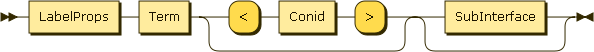
\includegraphics[resolution=120,max size={\textwidth}{\textheight}]
  {Figures/Ebnf/ObjDef}
  \caption*{ObjDef \small::=  LabelProps Term ('<' Conid '>')? SubInterface?}
  \label{fig:ebnf-ObjDef}
 \end{figure}

 \begin{figure}[H]
  \centering
  \includegraphics[resolution=120,max size={\textwidth}{\textheight}]
  {Figures/Ebnf/ObjDefList}
  \caption*{ObjDefList \small::=  ObjDef (',' ObjDef)*}
  \label{fig:ebnf-ObjDefList}
 \end{figure}

 \begin{figure}[H]
  \centering
  \includegraphics[resolution=120,max size={\textwidth}{\textheight}]
  {Figures/Ebnf/Box}
  \caption*{Box \small::=  '[' ObjDefList ']'}
  \label{fig:ebnf-Box}
 \end{figure}

 \begin{figure}[H]
  \centering
  \includegraphics[resolution=120,max size={\textwidth}{\textheight}]
  {Figures/Ebnf/Sqlplug}
  \caption*{Sqlplug \small::=  'SQLPLUG' ObjDef}
  \label{fig:ebnf-Sqlplug}
 \end{figure}

 \begin{figure}[H]
  \centering
  \includegraphics[resolution=120,max size={\textwidth}{\textheight}]
  {Figures/Ebnf/Phpplug}
  \caption*{Phpplug \small::=  'PHPPLUG' ObjDef}
  \label{fig:ebnf-Phpplug}
 \end{figure}

 \begin{figure}[H]
  \centering
  \includegraphics[resolution=120,max size={\textwidth}{\textheight}]
  {Figures/Ebnf/Purpose}
  \caption*{Purpose \small::=  'PURPOSE' Ref2Obj LanguageRef? TextMarkup? ('REF' StringListSemi)? Expl}
  \label{fig:ebnf-Purpose}
 \end{figure}

 \begin{figure}[H]
  \centering
  \includegraphics[resolution=120,max size={\textwidth}{\textheight}]
  {Figures/Ebnf/Ref2Obj}
  \caption*{Ref2Obj \small::=  'CONCEPT' ConceptName | 'RELATION' RelSign | 'RULE' ADLid | 'IDENT' ADLid | 'VIEW' ADLid | 'PATTERN' ADLid | 'PROCESS' ADLid | 'INTERFACE' ADLid | 'CONTEXT' ADLid}
  \label{fig:ebnf-Ref2Obj}
 \end{figure}

 \begin{figure}[H]
  \centering
  \includegraphics[resolution=120,max size={\textwidth}{\textheight}]
  {Figures/Ebnf/Population}
  \caption*{Population \small::=  'POPULATION' NamedRel 'CONTAINS' Content | 'POPULATION' ConceptName 'CONTAINS' '[' ValueList ']'}
  \label{fig:ebnf-Population}
 \end{figure}

 \begin{figure}[H]
  \centering
  \includegraphics[resolution=120,max size={\textwidth}{\textheight}]
  {Figures/Ebnf/RoleRelation}
  \caption*{RoleRelation \small::=  'ROLE' RoleList 'EDITS' NamedRelList}
  \label{fig:ebnf-RoleRelation}
 \end{figure}

 \begin{figure}[H]
  \centering
  \includegraphics[resolution=120,max size={\textwidth}{\textheight}]
  {Figures/Ebnf/RoleRule}
  \caption*{RoleRule \small::=  'ROLE' RoleList 'MAINTAINS' ADLidList}
  \label{fig:ebnf-RoleRule}
 \end{figure}

 \begin{figure}[H]
  \centering
  \includegraphics[resolution=120,max size={\textwidth}{\textheight}]
  {Figures/Ebnf/Role}
  \caption*{Role \small::=  ADLid}
  \label{fig:ebnf-Role}
 \end{figure}

 \begin{figure}[H]
  \centering
  \includegraphics[resolution=120,max size={\textwidth}{\textheight}]
  {Figures/Ebnf/RoleList}
  \caption*{RoleList \small::=  Role (',' Role)*}
  \label{fig:ebnf-RoleList}
 \end{figure}

 \begin{figure}[H]
  \centering
  \includegraphics[resolution=120,max size={\textwidth}{\textheight}]
  {Figures/Ebnf/PrintThemes}
  \caption*{PrintThemes \small::=  'THEMES' ConceptNameList}
  \label{fig:ebnf-PrintThemes}
 \end{figure}

 \begin{figure}[H]
  \centering
  \includegraphics[resolution=120,max size={\textwidth}{\textheight}]
  {Figures/Ebnf/Meaning}
  \caption*{Meaning \small::=  'MEANING' LanguageRef? TextMarkup? (String | Expl)}
  \label{fig:ebnf-Meaning}
 \end{figure}

 \begin{figure}[H]
  \centering
  \includegraphics[resolution=120,max size={\textwidth}{\textheight}]
  {Figures/Ebnf/Message}
  \caption*{Message \small::=  'MESSAGE' Markup}
  \label{fig:ebnf-Message}
 \end{figure}

 \begin{figure}[H]
  \centering
  \includegraphics[resolution=120,max size={\textwidth}{\textheight}]
  {Figures/Ebnf/Rule}
  \caption*{Rule \small::=  Term ('=' Term | '|-' Term)?}
  \label{fig:ebnf-Rule}
 \end{figure}

 \begin{figure}[H]
  \centering
  \includegraphics[resolution=120,max size={\textwidth}{\textheight}]
  {Figures/Ebnf/Term}
  \caption*{Term \small::=  Trm2 (('/\' Trm2)+ | ('\/' Trm2)+)?}
  \label{fig:ebnf-Term}
 \end{figure}

 \begin{figure}[H]
  \centering
  \includegraphics[resolution=120,max size={\textwidth}{\textheight}]
  {Figures/Ebnf/Trm2}
  \caption*{Trm2 \small::=  Trm3 ('-' Trm3)?}
  \label{fig:ebnf-Trm2}
 \end{figure}

 \begin{figure}[H]
  \centering
  \includegraphics[resolution=120,max size={\textwidth}{\textheight}]
  {Figures/Ebnf/Trm3}
  \caption*{Trm3 \small::=  Trm4 ('/' Trm4 | '\' Trm4 | '<>' Trm4)?}
  \label{fig:ebnf-Trm3}
 \end{figure}

 \begin{figure}[H]
  \centering
  \includegraphics[resolution=120,max size={\textwidth}{\textheight}]
  {Figures/Ebnf/Trm4}
  \caption*{Trm4 \small::=  Trm5 ((';' Trm5)+ | ('!' Trm5)+ | ('\#' Trm5)+)?}
  \label{fig:ebnf-Trm4}
 \end{figure}

 \begin{figure}[H]
  \centering
  \includegraphics[resolution=120,max size={\textwidth}{\textheight}]
  {Figures/Ebnf/Trm5}
  \caption*{Trm5 \small::=  '-'* Trm6 ('~' | '*' | '+')*}
  \label{fig:ebnf-Trm5}
 \end{figure}

 \begin{figure}[H]
  \centering
  \includegraphics[resolution=120,max size={\textwidth}{\textheight}]
  {Figures/Ebnf/Trm6}
  \caption*{Trm6 \small::=  RelationRef | '(' Term ')'}
  \label{fig:ebnf-Trm6}
 \end{figure}

 \begin{figure}[H]
  \centering
  \includegraphics[resolution=120,max size={\textwidth}{\textheight}]
  {Figures/Ebnf/RelationRef}
  \caption*{RelationRef \small::=  RelSign | 'I' ('[' ConceptOneRef ']')? | 'V' Sign? | Atom ('[' ConceptOneRef ']')?}
  \label{fig:ebnf-RelationRef}
 \end{figure}

 \begin{figure}[H]
  \centering
  \includegraphics[resolution=120,max size={\textwidth}{\textheight}]
  {Figures/Ebnf/NamedRelList}
  \caption*{NamedRelList \small::=  NamedRel (',' NamedRel)*}
  \label{fig:ebnf-NamedRelList}
 \end{figure}

 \begin{figure}[H]
  \centering
  \includegraphics[resolution=120,max size={\textwidth}{\textheight}]
  {Figures/Ebnf/NamedRel}
  \caption*{NamedRel \small::=  Varid Sign?}
  \label{fig:ebnf-NamedRel}
 \end{figure}

 \begin{figure}[H]
  \centering
  \includegraphics[resolution=120,max size={\textwidth}{\textheight}]
  {Figures/Ebnf/Sign}
  \caption*{Sign \small::=  '[' ConceptOneRef ('*' ConceptOneRef)? ']'}
  \label{fig:ebnf-Sign}
 \end{figure}

 \begin{figure}[H]
  \centering
  \includegraphics[resolution=120,max size={\textwidth}{\textheight}]
  {Figures/Ebnf/ConceptName}
  \caption*{ConceptName \small::=  Conid | String}
  \label{fig:ebnf-ConceptName}
 \end{figure}

 \begin{figure}[H]
  \centering
  \includegraphics[resolution=120,max size={\textwidth}{\textheight}]
  {Figures/Ebnf/ConceptNameList}
  \caption*{ConceptNameList \small::=  ConceptName (',' ConceptName)}
  \label{fig:ebnf-ConceptNameList}
 \end{figure}

 \begin{figure}[H]
  \centering
  \includegraphics[resolution=120,max size={\textwidth}{\textheight}]
  {Figures/Ebnf/ConceptRef}
  \caption*{ConceptRef \small::=  ConceptName}
  \label{fig:ebnf-ConceptRef}
 \end{figure}

 \begin{figure}[H]
  \centering
  \includegraphics[resolution=120,max size={\textwidth}{\textheight}]
  {Figures/Ebnf/ConceptOneRef}
  \caption*{ConceptOneRef \small::=  'ONE' | ConceptRef}
  \label{fig:ebnf-ConceptOneRef}
 \end{figure}

 \begin{figure}[H]
  \centering
  \includegraphics[resolution=120,max size={\textwidth}{\textheight}]
  {Figures/Ebnf/LabelProps}
  \caption*{LabelProps \small::=  ADLid ('{' ADLidListList '}')? ':'}
  \label{fig:ebnf-LabelProps}
 \end{figure}

 \begin{figure}[H]
  \centering
  \includegraphics[resolution=120,max size={\textwidth}{\textheight}]
  {Figures/Ebnf/Label}
  \caption*{Label \small::=  ADLid ':'}
  \label{fig:ebnf-Label}
 \end{figure}

 \begin{figure}[H]
  \centering
  \includegraphics[resolution=120,max size={\textwidth}{\textheight}]
  {Figures/Ebnf/Content}
  \caption*{Content \small::=  '[' RecordList? ']' | '[' RecordObsList? ']'}
  \label{fig:ebnf-Content}
 \end{figure}

 \begin{figure}[H]
  \centering
  \includegraphics[resolution=120,max size={\textwidth}{\textheight}]
  {Figures/Ebnf/RecordList}
  \caption*{RecordList \small::=  Record (',' Record)*}
  \label{fig:ebnf-RecordList}
 \end{figure}

 \begin{figure}[H]
  \centering
  \includegraphics[resolution=120,max size={\textwidth}{\textheight}]
  {Figures/Ebnf/Record}
  \caption*{Record \small::=  String '*' String}
  \label{fig:ebnf-Record}
 \end{figure}

 \begin{figure}[H]
  \centering
  \includegraphics[resolution=120,max size={\textwidth}{\textheight}]
  {Figures/Ebnf/RecordObsList}
  \caption*{RecordObsList \small::=  RecordObsList (';' RecordObsList)}
  \label{fig:ebnf-RecordObsList}
 \end{figure}

 \begin{figure}[H]
  \centering
  \includegraphics[resolution=120,max size={\textwidth}{\textheight}]
  {Figures/Ebnf/RecordObs}
  \caption*{RecordObs \small::=  '(' String ',' String ')'}
  \label{fig:ebnf-RecordObs}
 \end{figure}

 \begin{figure}[H]
  \centering
  \includegraphics[resolution=120,max size={\textwidth}{\textheight}]
  {Figures/Ebnf/ADLid}
  \caption*{ADLid \small::=  Varid | Conid | String}
  \label{fig:ebnf-ADLid}
 \end{figure}

 \begin{figure}[H]
  \centering
  \includegraphics[resolution=120,max size={\textwidth}{\textheight}]
  {Figures/Ebnf/ADLidList}
  \caption*{ADLidList \small::=  ADLid (',' ADLid)*}
  \label{fig:ebnf-ADLidList}
 \end{figure}

 \begin{figure}[H]
  \centering
  \includegraphics[resolution=120,max size={\textwidth}{\textheight}]
  {Figures/Ebnf/ADLidListList}
  \caption*{ADLidListList \small::=  ADLid+ (',' ADLid+)*}
  \label{fig:ebnf-ADLidListList}
 \end{figure}

 \begin{figure}[H]
  \centering
  \includegraphics[resolution=120,max size={\textwidth}{\textheight}]
  {Figures/Ebnf/Conid}
  \caption*{Conid \small::=  UpperChar (Char | '\_')*}
  \label{fig:ebnf-Conid}
 \end{figure}

 \begin{figure}[H]
  \centering
  \includegraphics[resolution=120,max size={\textwidth}{\textheight}]
  {Figures/Ebnf/String}
  \caption*{String \small::=  '"' Any* '"'}
  \label{fig:ebnf-String}
 \end{figure}

 \begin{figure}[H]
  \centering
  \includegraphics[resolution=120,max size={\textwidth}{\textheight}]
  {Figures/Ebnf/StringListSemi}
  \caption*{StringListSemi \small::=  String (';' String)*}
  \label{fig:ebnf-StringListSemi}
 \end{figure}

 \begin{figure}[H]
  \centering
  \includegraphics[resolution=120,max size={\textwidth}{\textheight}]
  {Figures/Ebnf/Expl}
  \caption*{Expl \small::=  '{+' Any* '-}'}
  \label{fig:ebnf-Expl}
 \end{figure}

 \begin{figure}[H]
  \centering
  \includegraphics[resolution=120,max size={\textwidth}{\textheight}]
  {Figures/Ebnf/Varid}
  \caption*{Varid \small::=  (LowerChar | '\_') (Char | '\_')*}
  \label{fig:ebnf-Varid}
 \end{figure}

